%% Orphans and Archetypes: paper version of the Mainz Hittite & AI workshop talk.
%% CEUR-WS template (ceurart), as used by the Computational Humanities Research (CHR) conference.
%% Build: bash build.sh  (regenerates every number from ../orphans/results, then lualatex + bibtex)
%%
%% Every result in the text is a macro \Q{key} defined in generated/numbers.tex and every results
%% table is generated/tab_*.tex; both are written by make_numbers.py. Do not type results by hand.
\documentclass{ceurart}

\sloppy
\usepackage{tabularx}
\usepackage{threeparttable}

%% numbers generated from the experiment outputs
\makeatletter
\newcommand{\qtmdef}[2]{\expandafter\def\csname qtm@#1\endcsname{#2}}
\newcommand{\Q}[1]{\ifcsname qtm@#1\endcsname\csname qtm@#1\endcsname\else
  \textbf{\textcolor{red}{[#1?]}}\PackageWarning{qtm}{Undefined number #1}\fi}
\makeatother
% generated by make_numbers.py from ../orphans/results; do not edit
\qtmdef{trad.count}{9}
\qtmdef{trad.countword}{nine}
\qtmdef{orph.cth470_texts}{1{,}919}
\qtmdef{orph.ebo_texts}{1{,}151}
\qtmdef{orph.orphans_total}{3{,}033}
\qtmdef{orph.cth470_median}{10}
\qtmdef{orph.ebo_median}{4}
\qtmdef{orph.ebo_832}{562}
\qtmdef{orph.ebo_670}{382}
\qtmdef{corpus.reference_texts}{3{,}282}
\qtmdef{corpus.orphans_used}{2{,}009}
\qtmdef{corpus.orphans_total}{2{,}898}
\qtmdef{corpus.orphan_median}{7}
\qtmdef{E1.words.acc}{82\%}
\qtmdef{E1.words.majority}{30\%}
\qtmdef{E1.words.null_mean}{16\%}
\qtmdef{E1.words.p}{0.005}
\qtmdef{E1.words.n}{1{,}596}
\qtmdef{E1.words.classes}{9}
\qtmdef{E1base.words.acc}{69\%}
\qtmdef{E1base.words.majority}{23\%}
\qtmdef{E1base.words.null_mean}{18\%}
\qtmdef{E1base.words.p}{0.005}
\qtmdef{E1base.words.n}{1{,}637}
\qtmdef{E1base.words.classes}{6}
\qtmdef{E1abs.words.acc}{88\%}
\qtmdef{E1abs.words.majority}{78\%}
\qtmdef{E1abs.words.null_mean}{53\%}
\qtmdef{E1abs.words.p}{0.005}
\qtmdef{E1abs.words.n}{1{,}254}
\qtmdef{E1abs.words.classes}{3}
\qtmdef{E1.signs.acc}{84\%}
\qtmdef{E1.signs.majority}{30\%}
\qtmdef{E1.signs.null_mean}{16\%}
\qtmdef{E1.signs.p}{0.005}
\qtmdef{E1.signs.n}{1{,}596}
\qtmdef{E1.signs.classes}{9}
\qtmdef{E1base.signs.acc}{72\%}
\qtmdef{E1base.signs.majority}{23\%}
\qtmdef{E1base.signs.null_mean}{18\%}
\qtmdef{E1base.signs.p}{0.005}
\qtmdef{E1base.signs.n}{1{,}637}
\qtmdef{E1base.signs.classes}{6}
\qtmdef{E1abs.signs.acc}{89\%}
\qtmdef{E1abs.signs.majority}{78\%}
\qtmdef{E1abs.signs.null_mean}{53\%}
\qtmdef{E1abs.signs.p}{0.005}
\qtmdef{E1abs.signs.n}{1{,}254}
\qtmdef{E1abs.signs.classes}{3}
\qtmdef{E1.both.acc}{84\%}
\qtmdef{E1.both.majority}{30\%}
\qtmdef{E1.both.null_mean}{17\%}
\qtmdef{E1.both.p}{0.005}
\qtmdef{E1.both.n}{1{,}596}
\qtmdef{E1.both.classes}{9}
\qtmdef{E1base.both.acc}{72\%}
\qtmdef{E1base.both.majority}{23\%}
\qtmdef{E1base.both.null_mean}{18\%}
\qtmdef{E1base.both.p}{0.005}
\qtmdef{E1base.both.n}{1{,}637}
\qtmdef{E1base.both.classes}{6}
\qtmdef{E1abs.both.acc}{89\%}
\qtmdef{E1abs.both.majority}{78\%}
\qtmdef{E1abs.both.null_mean}{55\%}
\qtmdef{E1abs.both.p}{0.005}
\qtmdef{E1abs.both.n}{1{,}254}
\qtmdef{E1abs.both.classes}{3}
\qtmdef{E4.words.acc}{76\%}
\qtmdef{E4.words.majority}{30\%}
\qtmdef{E4.words.null_mean}{16\%}
\qtmdef{E4.words.p}{0.005}
\qtmdef{E4.words.n}{1{,}596}
\qtmdef{E4.words.classes}{9}
\qtmdef{E4.signs.acc}{81\%}
\qtmdef{E4.signs.majority}{30\%}
\qtmdef{E4.signs.null_mean}{16\%}
\qtmdef{E4.signs.p}{0.005}
\qtmdef{E4.signs.n}{1{,}596}
\qtmdef{E4.signs.classes}{9}
\qtmdef{trad.kizzuwatnalowerlandhurrian.n}{311}
\qtmdef{trad.kizzuwatnalowerlandhurrian.recall}{83\%}
\qtmdef{trad.kizzuwatnalowerlandhurrian.orphans}{71}
\qtmdef{trad.kizzuwatnalowerlandhurrian.coverage}{93\%}
\qtmdef{trad.syromesopotamiahurrian.n}{164}
\qtmdef{trad.syromesopotamiahurrian.recall}{67\%}
\qtmdef{trad.syromesopotamiahurrian.orphans}{58}
\qtmdef{trad.syromesopotamiahurrian.coverage}{92\%}
\qtmdef{trad.mixedhurriansyrianluwian.n}{198}
\qtmdef{trad.mixedhurriansyrianluwian.recall}{67\%}
\qtmdef{trad.mixedhurriansyrianluwian.orphans}{25}
\qtmdef{trad.mixedhurriansyrianluwian.coverage}{67\%}
\qtmdef{trad.luwianfestivalsistanuwalallupiya.n}{50}
\qtmdef{trad.luwianfestivalsistanuwalallupiya.recall}{84\%}
\qtmdef{trad.luwianfestivalsistanuwalallupiya.orphans}{8}
\qtmdef{trad.luwianfestivalsistanuwalallupiya.coverage}{57\%}
\qtmdef{trad.huwassannafestivals.n}{180}
\qtmdef{trad.huwassannafestivals.recall}{91\%}
\qtmdef{trad.huwassannafestivals.orphans}{14}
\qtmdef{trad.huwassannafestivals.coverage}{56\%}
\qtmdef{trad.palaicfestivals.n}{34}
\qtmdef{trad.palaicfestivals.recall}{82\%}
\qtmdef{trad.palaicfestivals.orphans}{4}
\qtmdef{trad.palaicfestivals.coverage}{34\%}
\qtmdef{trad.kizzuwatnarituals.n}{164}
\qtmdef{trad.kizzuwatnarituals.recall}{92\%}
\qtmdef{trad.kizzuwatnarituals.orphans}{529}
\qtmdef{trad.kizzuwatnarituals.coverage}{100\%}
\qtmdef{trad.arzawawesternrituals.n}{17}
\qtmdef{trad.arzawawesternrituals.recall}{41\%}
\qtmdef{trad.arzawawesternrituals.orphans}{25}
\qtmdef{trad.arzawawesternrituals.coverage}{76\%}
\qtmdef{trad.hattiancultlayer.n}{478}
\qtmdef{trad.hattiancultlayer.recall}{95\%}
\qtmdef{trad.hattiancultlayer.orphans}{134}
\qtmdef{trad.hattiancultlayer.coverage}{98\%}
\qtmdef{trad.minrecall}{41\%}
\qtmdef{trad.maxrecall}{95\%}
\qtmdef{trad.smallest}{Arzawa / western rituals}
\qtmdef{trad.smallest.n}{17}
\qtmdef{E2.both.k3}{51\%}
\qtmdef{E2.both.k5}{59\%}
\qtmdef{E2.both.k8}{64\%}
\qtmdef{E2.both.k10}{66\%}
\qtmdef{E2.both.k17}{71\%}
\qtmdef{E2.both.k25}{74\%}
\qtmdef{E2.both.k40}{78\%}
\qtmdef{E2.signs.k3}{49\%}
\qtmdef{E2.signs.k5}{57\%}
\qtmdef{E2.signs.k8}{63\%}
\qtmdef{E2.signs.k10}{65\%}
\qtmdef{E2.signs.k17}{70\%}
\qtmdef{E2.signs.k25}{74\%}
\qtmdef{E2.signs.k40}{78\%}
\qtmdef{E2.words.k3}{47\%}
\qtmdef{E2.words.k5}{54\%}
\qtmdef{E2.words.k8}{60\%}
\qtmdef{E2.words.k10}{62\%}
\qtmdef{E2.words.k17}{69\%}
\qtmdef{E2.words.k25}{72\%}
\qtmdef{E2.words.k40}{77\%}
\qtmdef{E2.margin}{0.017}
\qtmdef{E2.margin.lo}{0.016}
\qtmdef{E2.margin.hi}{0.017}
\qtmdef{E2.precision}{81\%}
\qtmdef{E2.share}{67\%}
\qtmdef{chance}{11\%}
\qtmdef{E3.words.acc}{50\%}
\qtmdef{E3.words.majority}{21\%}
\qtmdef{E3.words.null_mean}{14\%}
\qtmdef{E3.words.p}{0.005}
\qtmdef{E3.words.n}{82}
\qtmdef{E3.words.classes}{8}
\qtmdef{E3date.words.acc}{73\%}
\qtmdef{E3date.words.majority}{83\%}
\qtmdef{E3date.words.null_mean}{71\%}
\qtmdef{E3date.words.p}{0.4129}
\qtmdef{E3date.words.n}{99}
\qtmdef{E3date.words.classes}{2}
\qtmdef{E3.signs.acc}{60\%}
\qtmdef{E3.signs.majority}{21\%}
\qtmdef{E3.signs.null_mean}{14\%}
\qtmdef{E3.signs.p}{0.005}
\qtmdef{E3.signs.n}{82}
\qtmdef{E3.signs.classes}{8}
\qtmdef{E3date.signs.acc}{74\%}
\qtmdef{E3date.signs.majority}{83\%}
\qtmdef{E3date.signs.null_mean}{72\%}
\qtmdef{E3date.signs.p}{0.4229}
\qtmdef{E3date.signs.n}{99}
\qtmdef{E3date.signs.classes}{2}
\qtmdef{E3.both.acc}{58\%}
\qtmdef{E3.both.majority}{21\%}
\qtmdef{E3.both.null_mean}{14\%}
\qtmdef{E3.both.p}{0.005}
\qtmdef{E3.both.n}{82}
\qtmdef{E3.both.classes}{8}
\qtmdef{E3date.both.acc}{74\%}
\qtmdef{E3date.both.majority}{83\%}
\qtmdef{E3date.both.null_mean}{73\%}
\qtmdef{E3date.both.p}{0.4527}
\qtmdef{E3date.both.n}{99}
\qtmdef{E3date.both.classes}{2}
\qtmdef{E3.unclassified}{50}
\qtmdef{E5.assigned}{868}
\qtmdef{E5.abstained}{1{,}141}
\qtmdef{E5.assigned.lo}{868}
\qtmdef{E5.assigned.hi}{925}
\qtmdef{E5.top}{Kizzuwatna rituals}
\qtmdef{E5.top.n}{529}
\qtmdef{E5.top.share}{61\%}
\qtmdef{E5b.res.texts}{300}
\qtmdef{E5b.res.assigned}{164}
\qtmdef{E5b.res.kizz}{141}
\qtmdef{E5b.res.hurrian}{4}
\qtmdef{E5b.c500.texts}{235}
\qtmdef{E5b.c500.assigned}{125}
\qtmdef{E5b.c500.kizz}{52}
\qtmdef{E5b.c500.hurrian}{72}
\qtmdef{E7.logograms.acc}{70\%}
\qtmdef{E7.logograms.majority}{28\%}
\qtmdef{E7.logograms.null_mean}{14\%}
\qtmdef{E7.logograms.p}{0.0099}
\qtmdef{E7.logograms.n}{1{,}531}
\qtmdef{E7.logograms.classes}{9}
\qtmdef{E7.lexicon.acc}{72\%}
\qtmdef{E7.lexicon.majority}{27\%}
\qtmdef{E7.lexicon.null_mean}{16\%}
\qtmdef{E7.lexicon.p}{0.0099}
\qtmdef{E7.lexicon.n}{1{,}526}
\qtmdef{E7.lexicon.classes}{9}
\qtmdef{E7.foreign.acc}{88\%}
\qtmdef{E7.foreign.majority}{50\%}
\qtmdef{E7.foreign.null_mean}{24\%}
\qtmdef{E7.foreign.p}{0.0099}
\qtmdef{E7.foreign.n}{396}
\qtmdef{E7.foreign.classes}{8}
\qtmdef{E7.collapsed.acc}{62\%}
\qtmdef{E7.collapsed.majority}{28\%}
\qtmdef{E7.collapsed.null_mean}{12\%}
\qtmdef{E7.collapsed.p}{0.0099}
\qtmdef{E7.collapsed.n}{1{,}508}
\qtmdef{E7.collapsed.classes}{9}
\qtmdef{E7.spelling.acc}{62\%}
\qtmdef{E7.spelling.majority}{28\%}
\qtmdef{E7.spelling.null_mean}{13\%}
\qtmdef{E7.spelling.p}{0.0099}
\qtmdef{E7.spelling.n}{1{,}504}
\qtmdef{E7.spelling.classes}{9}
\qtmdef{E7.orthographic_indices.acc}{39\%}
\qtmdef{E7.orthographic_indices.majority}{30\%}
\qtmdef{E7.orthographic_indices.null_mean}{30\%}
\qtmdef{E7.orthographic_indices.p}{0.0099}
\qtmdef{E7.orthographic_indices.n}{1{,}597}
\qtmdef{E7.orthographic_indices.classes}{9}
\qtmdef{E7.variable_words}{384}
\qtmdef{E7.texts}{1{,}597}
\qtmdef{E7date.acc}{75\%}
\qtmdef{E7date.majority}{83\%}
\qtmdef{plene.akuanzi.arzawawesternrituals}{0 of 1}
\qtmdef{plene.akuanzi.arzawawesternrituals.cths}{--}
\qtmdef{plene.akuanzi.hattiancultlayer}{0 of 53}
\qtmdef{plene.akuanzi.hattiancultlayer.cths}{--}
\qtmdef{plene.akuanzi.kizzuwatnalowerlandhurrian}{0 of 9}
\qtmdef{plene.akuanzi.kizzuwatnalowerlandhurrian.cths}{--}
\qtmdef{plene.akuanzi.luwianfestivalsistanuwalallupiya}{0 of 14}
\qtmdef{plene.akuanzi.luwianfestivalsistanuwalallupiya.cths}{--}
\qtmdef{plene.akuanzi.mixedhurriansyrianluwian}{0 of 2}
\qtmdef{plene.akuanzi.mixedhurriansyrianluwian.cths}{--}
\qtmdef{plene.akuanzi.syromesopotamiahurrian}{0 of 2}
\qtmdef{plene.akuanzi.syromesopotamiahurrian.cths}{--}
\qtmdef{plene.akuanzi.huwassannafestivals}{1 of 52}
\qtmdef{plene.akuanzi.huwassannafestivals.cths}{694}
\qtmdef{plene.memai.arzawawesternrituals}{0 of 2}
\qtmdef{plene.memai.arzawawesternrituals.cths}{--}
\qtmdef{plene.memai.hattiancultlayer}{10 of 79}
\qtmdef{plene.memai.hattiancultlayer.cths}{591, 627, 733, 820}
\qtmdef{plene.memai.kizzuwatnarituals}{2 of 47}
\qtmdef{plene.memai.kizzuwatnarituals.cths}{474, 490}
\qtmdef{plene.memai.kizzuwatnalowerlandhurrian}{18 of 46}
\qtmdef{plene.memai.kizzuwatnalowerlandhurrian.cths}{628, 712}
\qtmdef{plene.memai.luwianfestivalsistanuwalallupiya}{0 of 3}
\qtmdef{plene.memai.luwianfestivalsistanuwalallupiya.cths}{--}
\qtmdef{plene.memai.mixedhurriansyrianluwian}{1 of 8}
\qtmdef{plene.memai.mixedhurriansyrianluwian.cths}{705}
\qtmdef{plene.memai.palaicfestivals}{0 of 7}
\qtmdef{plene.memai.palaicfestivals.cths}{--}
\qtmdef{plene.memai.syromesopotamiahurrian}{3 of 72}
\qtmdef{plene.memai.syromesopotamiahurrian.cths}{701}
\qtmdef{plene.memai.huwassannafestivals}{0 of 8}
\qtmdef{plene.memai.huwassannafestivals.cths}{--}
\qtmdef{plene.peran.arzawawesternrituals}{0 of 3}
\qtmdef{plene.peran.arzawawesternrituals.cths}{--}
\qtmdef{plene.peran.hattiancultlayer}{12 of 118}
\qtmdef{plene.peran.hattiancultlayer.cths}{627, 731, 744, 820}
\qtmdef{plene.peran.kizzuwatnarituals}{0 of 31}
\qtmdef{plene.peran.kizzuwatnarituals.cths}{--}
\qtmdef{plene.peran.kizzuwatnalowerlandhurrian}{0 of 56}
\qtmdef{plene.peran.kizzuwatnalowerlandhurrian.cths}{--}
\qtmdef{plene.peran.luwianfestivalsistanuwalallupiya}{5 of 19}
\qtmdef{plene.peran.luwianfestivalsistanuwalallupiya.cths}{665}
\qtmdef{plene.peran.mixedhurriansyrianluwian}{0 of 34}
\qtmdef{plene.peran.mixedhurriansyrianluwian.cths}{--}
\qtmdef{plene.peran.palaicfestivals}{0 of 4}
\qtmdef{plene.peran.palaicfestivals.cths}{--}
\qtmdef{plene.peran.syromesopotamiahurrian}{0 of 39}
\qtmdef{plene.peran.syromesopotamiahurrian.cths}{--}
\qtmdef{plene.peran.huwassannafestivals}{0 of 24}
\qtmdef{plene.peran.huwassannafestivals.cths}{--}
\qtmdef{plene.šer.arzawawesternrituals}{0 of 3}
\qtmdef{plene.šer.arzawawesternrituals.cths}{--}
\qtmdef{plene.šer.hattiancultlayer}{6 of 54}
\qtmdef{plene.šer.hattiancultlayer.cths}{627, 736, 738, 744}
\qtmdef{plene.šer.kizzuwatnarituals}{0 of 33}
\qtmdef{plene.šer.kizzuwatnarituals.cths}{--}
\qtmdef{plene.šer.kizzuwatnalowerlandhurrian}{2 of 52}
\qtmdef{plene.šer.kizzuwatnalowerlandhurrian.cths}{713}
\qtmdef{plene.šer.luwianfestivalsistanuwalallupiya}{0 of 5}
\qtmdef{plene.šer.luwianfestivalsistanuwalallupiya.cths}{--}
\qtmdef{plene.šer.mixedhurriansyrianluwian}{0 of 23}
\qtmdef{plene.šer.mixedhurriansyrianluwian.cths}{--}
\qtmdef{plene.šer.palaicfestivals}{2 of 9}
\qtmdef{plene.šer.palaicfestivals.cths}{752}
\qtmdef{plene.šer.syromesopotamiahurrian}{0 of 26}
\qtmdef{plene.šer.syromesopotamiahurrian.cths}{--}
\qtmdef{plene.šer.huwassannafestivals}{0 of 18}
\qtmdef{plene.šer.huwassannafestivals.cths}{--}
\qtmdef{plene.ḫalzai.hattiancultlayer}{74 of 78}
\qtmdef{plene.ḫalzai.hattiancultlayer.cths}{591, 627, 734, 738, 739, 741, 743, 744}
\qtmdef{plene.ḫalzai.kizzuwatnarituals}{11 of 13}
\qtmdef{plene.ḫalzai.kizzuwatnarituals.cths}{477, 483, 488, 490, 494}
\qtmdef{plene.ḫalzai.kizzuwatnalowerlandhurrian}{6 of 6}
\qtmdef{plene.ḫalzai.kizzuwatnalowerlandhurrian.cths}{699, 711, 712}
\qtmdef{plene.ḫalzai.luwianfestivalsistanuwalallupiya}{2 of 2}
\qtmdef{plene.ḫalzai.luwianfestivalsistanuwalallupiya.cths}{665, 771}
\qtmdef{plene.ḫalzai.mixedhurriansyrianluwian}{6 of 6}
\qtmdef{plene.ḫalzai.mixedhurriansyrianluwian.cths}{704, 705, 706}
\qtmdef{plene.ḫalzai.syromesopotamiahurrian}{1 of 1}
\qtmdef{plene.ḫalzai.syromesopotamiahurrian.cths}{701}
\qtmdef{plene.ḫalzai.huwassannafestivals}{7 of 7}
\qtmdef{plene.ḫalzai.huwassannafestivals.cths}{691, 692, 694}
\qtmdef{E8.all.words}{82\%}
\qtmdef{E8.all.signs}{84\%}
\qtmdef{E8.only_agent.words}{53\%}
\qtmdef{E8.only_agent.signs}{61\%}
\qtmdef{E8.only_agent.majority}{31\%}
\qtmdef{E8.without_agent.words}{81\%}
\qtmdef{E8.without_agent.signs}{83\%}
\qtmdef{E8.without_agent.majority}{30\%}
\qtmdef{E8.only_deity.words}{60\%}
\qtmdef{E8.only_deity.signs}{60\%}
\qtmdef{E8.only_deity.majority}{24\%}
\qtmdef{E8.without_deity.words}{80\%}
\qtmdef{E8.without_deity.signs}{82\%}
\qtmdef{E8.without_deity.majority}{30\%}
\qtmdef{E8.only_function.words}{58\%}
\qtmdef{E8.only_function.signs}{58\%}
\qtmdef{E8.only_function.majority}{27\%}
\qtmdef{E8.without_function.words}{81\%}
\qtmdef{E8.without_function.signs}{84\%}
\qtmdef{E8.without_function.majority}{30\%}
\qtmdef{E8.only_verb.words}{56\%}
\qtmdef{E8.only_verb.signs}{54\%}
\qtmdef{E8.only_verb.majority}{27\%}
\qtmdef{E8.without_verb.words}{81\%}
\qtmdef{E8.without_verb.signs}{84\%}
\qtmdef{E8.without_verb.majority}{30\%}
\qtmdef{E8.only_realia.words}{71\%}
\qtmdef{E8.only_realia.signs}{73\%}
\qtmdef{E8.only_realia.majority}{27\%}
\qtmdef{E8.without_realia.words}{76\%}
\qtmdef{E8.without_realia.signs}{79\%}
\qtmdef{E8.without_realia.majority}{30\%}
\qtmdef{E8.only_foreign.words}{87\%}
\qtmdef{E8.only_foreign.signs}{89\%}
\qtmdef{E8.only_foreign.majority}{49\%}
\qtmdef{E8.without_foreign.words}{78\%}
\qtmdef{E8.without_foreign.signs}{80\%}
\qtmdef{E8.without_foreign.majority}{28\%}
\qtmdef{E8.701.all.words}{50\%}
\qtmdef{E8.701.all.majority}{21\%}
\qtmdef{E8.701.without_foreign.words}{47\%}
\qtmdef{E8.701.without_foreign.majority}{20\%}
\qtmdef{E8.701.only_foreign.words}{54\%}
\qtmdef{E8.701.only_foreign.majority}{19\%}
\qtmdef{E9.k}{10}
\qtmdef{E9.ref.placed}{70\%}
\qtmdef{E9.ref.correct}{83\%}
\qtmdef{E9.ref.gate}{21\%}
\qtmdef{E9.genres.placed.lo}{23\%}
\qtmdef{E9.genres.placed.hi}{31\%}
\qtmdef{E9.genres.gate.lo}{87\%}
\qtmdef{E9.genres.gate.hi}{97\%}
\qtmdef{E9.genres.auroc.lo}{0.77}
\qtmdef{E9.genres.auroc.hi}{0.88}
\qtmdef{E9.fest.placed}{59\%}
\qtmdef{E9.fest.auroc}{0.57}
\qtmdef{E9.fest.gate}{66\%}
\qtmdef{E9.genres.count}{six}
\qtmdef{E9.orph.scored}{2{,}009}
\qtmdef{E9.orph.outside}{247}
\qtmdef{E9.orph.assigned_outside}{85}
\qtmdef{E9.orph.below_floor}{156}
\qtmdef{E9.orph.arzawawesternrituals.cultinventories}{0}
\qtmdef{E9.orph.arzawawesternrituals.festivalsofothertraditions}{0}
\qtmdef{E9.orph.arzawawesternrituals.historicaltextstreaties}{0}
\qtmdef{E9.orph.arzawawesternrituals.instructions}{0}
\qtmdef{E9.orph.arzawawesternrituals.luwianritualspuriyannikuwattalla}{0}
\qtmdef{E9.orph.arzawawesternrituals.myths}{1}
\qtmdef{E9.orph.arzawawesternrituals.oracles}{0}
\qtmdef{E9.orph.hattiancultlayer.cultinventories}{0}
\qtmdef{E9.orph.hattiancultlayer.festivalsofothertraditions}{30}
\qtmdef{E9.orph.hattiancultlayer.historicaltextstreaties}{3}
\qtmdef{E9.orph.hattiancultlayer.instructions}{0}
\qtmdef{E9.orph.hattiancultlayer.luwianritualspuriyannikuwattalla}{1}
\qtmdef{E9.orph.hattiancultlayer.myths}{0}
\qtmdef{E9.orph.hattiancultlayer.oracles}{0}
\qtmdef{E9.orph.kizzuwatnarituals.cultinventories}{5}
\qtmdef{E9.orph.kizzuwatnarituals.festivalsofothertraditions}{0}
\qtmdef{E9.orph.kizzuwatnarituals.historicaltextstreaties}{5}
\qtmdef{E9.orph.kizzuwatnarituals.instructions}{10}
\qtmdef{E9.orph.kizzuwatnarituals.luwianritualspuriyannikuwattalla}{5}
\qtmdef{E9.orph.kizzuwatnarituals.myths}{10}
\qtmdef{E9.orph.kizzuwatnarituals.oracles}{1}
\qtmdef{E9.orph.kizzuwatnalowerlandhurrian.cultinventories}{10}
\qtmdef{E9.orph.kizzuwatnalowerlandhurrian.festivalsofothertraditions}{0}
\qtmdef{E9.orph.kizzuwatnalowerlandhurrian.historicaltextstreaties}{0}
\qtmdef{E9.orph.kizzuwatnalowerlandhurrian.instructions}{0}
\qtmdef{E9.orph.kizzuwatnalowerlandhurrian.luwianritualspuriyannikuwattalla}{0}
\qtmdef{E9.orph.kizzuwatnalowerlandhurrian.myths}{0}
\qtmdef{E9.orph.kizzuwatnalowerlandhurrian.oracles}{0}
\qtmdef{E9.orph.luwianfestivalsistanuwalallupiya.cultinventories}{1}
\qtmdef{E9.orph.luwianfestivalsistanuwalallupiya.festivalsofothertraditions}{0}
\qtmdef{E9.orph.luwianfestivalsistanuwalallupiya.historicaltextstreaties}{0}
\qtmdef{E9.orph.luwianfestivalsistanuwalallupiya.instructions}{0}
\qtmdef{E9.orph.luwianfestivalsistanuwalallupiya.luwianritualspuriyannikuwattalla}{0}
\qtmdef{E9.orph.luwianfestivalsistanuwalallupiya.myths}{0}
\qtmdef{E9.orph.luwianfestivalsistanuwalallupiya.oracles}{0}
\qtmdef{E9.orph.mixedhurriansyrianluwian.cultinventories}{0}
\qtmdef{E9.orph.mixedhurriansyrianluwian.festivalsofothertraditions}{0}
\qtmdef{E9.orph.mixedhurriansyrianluwian.historicaltextstreaties}{0}
\qtmdef{E9.orph.mixedhurriansyrianluwian.instructions}{0}
\qtmdef{E9.orph.mixedhurriansyrianluwian.luwianritualspuriyannikuwattalla}{3}
\qtmdef{E9.orph.mixedhurriansyrianluwian.myths}{0}
\qtmdef{E9.orph.mixedhurriansyrianluwian.oracles}{0}

%% results tables; the primitive \input is expandable, so a table body can follow \midrule
\makeatletter\newcommand{\gentab}[1]{\@@input generated/tab_#1.tex }\makeatother

\graphicspath{{../img/orphans/literature/}}
\newcommand{\CTH}[1]{CTH~#1}
\newcommand{\term}[1]{\textit{#1}}

\begin{document}

\copyrightyear{2026}
\copyrightclause{Copyright for this paper by its authors.
  Use permitted under Creative Commons License Attribution 4.0 International (CC BY 4.0).}

\conference{Hittite and Artificial Intelligence workshop, Mainz, November 2026 (draft in CHR/CEUR-WS format)}

\title{Orphans and Archetypes: Linking Unidentified Ritual Fragments to {H}ittite Textual Traditions
  through Quantitative Scribal Tradition Mapping}

\author[1,2]{Shai Gordin}
\address[1]{Ariel University, Israel}
\address[2]{Open University of Israel}

\begin{abstract}
  The Hittite ritual corpus contains a large body of manuscript fragments that resist
  classification within established textual traditions: Laroche's residual category \CTH{470}
  and the newly digitised EBo fragments, \Q{orph.orphans_total} manuscripts in the TLHdig 0.3
  release, with a median of \Q{orph.cth470_median} (\CTH{470}) and \Q{orph.ebo_median} (EBo)
  legible words. Philological assignment needs a parallel passage, which these ``orphans''
  lack. We treat tradition assignment as a content-based classification problem. Word tf-idf
  and orthographic sign n-gram features from TLHdig define a reference space of
  \Q{trad.countword} ritual and festival traditions, each delimited by the study that argued
  for it and mapped back to Laroche's CTH numbers. A held-out manuscript is assigned to its
  correct tradition in \Q{E1.both.acc} of cases (majority baseline \Q{E1.both.majority}), and
  a ten-word window in \Q{E2.both.k10}. Separating the layers of a text shows that traditions
  are identified by what is written (logograms, Hittite vocabulary, foreign-language words),
  not by how it is written: spelling adds nothing beyond the words, and orthographic rates
  carry only a weak signal that follows compositions and their copies. On \CTH{701}, where
  Salvini and Wegner's subgroups provide partial ground truth, the method recovers
  \Q{E3.both.acc} of subgroup labels (majority \Q{E3.both.majority}) and does not predict
  script date. When whole compositions are held out, \Q{E10a.compositions_correct} of
  \Q{E10a.compositions} return to their scholarly group: the Hattian, Ḫuwaššanna and Kizzuwatna
  groups are recovered, the Hurrian festival groups and Palaic are not. With a calibrated abstention margin, \Q{E5.assigned} of \Q{corpus.orphans_used}
  orphans are placed; an open-set test shows that a closed reference must be paired with
  explicit outside classes before such placements can be read as ``this tradition''. We
  interpret the results through Quantitative Scribal Tradition Mapping (QTM), which treats
  orphans as low-coverage witnesses to incompletely attested archetypes.
\end{abstract}

\begin{keywords}
  Hittite \sep
  cuneiform \sep
  stylometry \sep
  fragment attribution \sep
  open-set recognition \sep
  textual traditions \sep
  digital philology
\end{keywords}

\maketitle

%% ==========================================================================================
\section{Introduction}
\label{sec:intro}

Emmanuel Laroche's \textit{Catalogue des textes hittites} \cite{laroche1971catalogue} gave every
Hittite composition a number, and with it a place: rituals in one block, festivals in another,
texts in Hattian, Luwian and Hurrian in blocks of their own. What could not be placed went into
residual categories. \CTH{470}, ``fragments of rituals'', is the largest of them, and it has
grown with every volume of hand copies since 1971. The Mainz Hethitologie-Portal now keeps
Laroche's numbers as a shared address system while moving fragments after joins and adding new
texts \cite{cthportal,konkordanz}. The digitisation of the EBo fragments in TLHdig 0.3
\cite{tlhdig03} adds \Q{orph.ebo_texts} more manuscripts with a median of
\Q{orph.ebo_median} legible words, most of them filed under \CTH{832} (\Q{orph.ebo_832}) and
\CTH{670} (\Q{orph.ebo_670}), two further residual categories.

The philological route to assigning such a fragment runs through a parallel: a duplicate or a
close parallel passage in an identified composition. That route is closed for most orphans by
definition. This paper asks whether the content of a fragment, its words and the way they are
spelled, can point to its tradition instead, and how far such a pointer can be trusted. It
builds on an exploratory study of the Hurrian and Luwian festival texts
\cite{gordin2025matters}, which mapped about 1,000 manuscripts with tf-idf and t-SNE, examined
\CTH{701} under the ``microscope'', and announced as its next step the test of which word groups
carry the signal. Here the exploration becomes assignment, with explicit baselines, held-out
evaluation and a rule for when not to assign.

Our contributions are:
\begin{enumerate}
  \item a reference space of \Q{trad.countword} Hittite ritual and festival traditions, each
    defined by the study that argued for it and mapped back to Laroche's CTH numbers, with
    the CTH ranges that no study claims set aside as test sets (Section~\ref{sec:data});
  \item a validation of nearest-centroid tradition assignment against majority and permutation
    baselines, as a function of fragment size, and on \CTH{701}, where partial ground truth
    exists, and a leave-one-composition-out test of the scholarly groups themselves
    (Sections~\ref{sec:validation}--\ref{sec:cth701});
  \item a decomposition of the signal into layers and word classes that separates what is
    written (cultural content) from how it is written (scribal habit), and an exact split of
    each decision over them, which shows how much rests on common particles such as \textit{nu}
    (Sections~\ref{sec:layers}--\ref{sec:decision});
  \item a placement of the \CTH{470} and EBo orphans with a calibrated abstention margin, and an
    open-set test of whether the method notices a fragment that belongs to no reference
    tradition (Sections~\ref{sec:orphans}--\ref{sec:openset});
  \item Quantitative Scribal Tradition Mapping (QTM), a framework that reads the results in
    terms of witnesses and archetypes (Section~\ref{sec:qtm}).
\end{enumerate}
All code, the label snapshot and the outputs are public, and every number in this paper is
generated from the experiment outputs (Section~\ref{sec:availability}).

%% ==========================================================================================
\section{Background and related work}
\label{sec:related}

\paragraph{Traditions and the catalogue.}
Laroche's catalogue sorts by genre first and by language second, while later scholarship
defines a ritual tradition by the origin of its practitioners, its cult and its ritual
language. One tradition therefore ends up scattered over several CTH ranges. The Kizzuwatna
rituals occupy \CTH{471}--500, but the ritual of the Kizzuwatnean Old Woman Maštigga is filed
with the named practitioners at \CTH{404} \cite{miller2004studies}; the rituals of the AZU
priest (\CTH{701}) sit in the Hurrian block rather than with the Kizzuwatna rituals
\cite{salvini1986chs}; and the named-practitioner rituals of \CTH{390}--469 come from Arzawa,
the Lower Land and Kizzuwatna alike \cite{christiansen2006ambazzi,bawanypeck2005auguren}. The
festival texts have been regrouped by cult geography \cite{gordin2025matters,gorke2022hurrian,
trameri2024kizzuwatna} and, in the Hethitische Festrituale (HFR) project, into edition modules
such as the Luwian and the Palaic festivals \cite{hfr,gorke2020hatti}. Surveys of Hittite
religion frame all of these \cite{haas1994geschichte,taracha2009religions}.

\paragraph{Scribal habit and its measurement.}
Hittite scribes copied, excerpted and re-edited ritual texts over two centuries, and their
writing habits (logographic writing, plene spelling, sign choice) vary with date, school and
individual \cite{gordin2015scribal,weeden2011logograms,vandenhout2009dating,
vandenhout2020literacy,waal2015diplomatics}. Whether a habit marks a tradition, a scribal circle
or a date is therefore an empirical question, and one this paper tests rather than assumes.
Stylometry offers the tools: frequency-based representations, distance measures and
attribution protocols with held-out evaluation \cite{burrows2002delta,juola2008authorship,
stamatatos2009survey}. Two of its known problems are central here. Short samples degrade
attribution sharply \cite{eder2015size}, and a closed-set classifier always names one of its
candidates, even when the true author is not among them \cite{koppel2011wild}; the latter is
the problem of open-set recognition \cite{scheirer2013openset}.

\paragraph{Computational work on cuneiform.}
Machine learning on cuneiform has addressed transliteration and translation
\cite{gordin2020reading,yavasan2025clay}, language and dialect identification
\cite{jauhiainen2019cuneiform}, the matching of fragments to known compositions by sign
sequences \cite{simonjetz2024reconstruction}, and palaeographic style
\cite{yugay2024stylistic}. Fragment matching finds a known text; it does not place a fragment
whose parallels are lost. All of these studies are closed-set. To our knowledge, no published
study uses content features to assign Hittite fragments to religious traditions, or asks when a
fragment fits none of the candidates.

%% ==========================================================================================
\section{Data}
\label{sec:data}

\paragraph{Corpus.}
We use the TLHdig Beta 0.3 release \cite{tlhdig03}, converted to one row per word following
\cite{yavasan2025clay}. Each word carries its normalised form, its transliteration split into
signs, its language layer and, where TLHdig provides a morphological analysis, a word class. The
release is downloaded by script and checked by its MD5 sum, so the token table can be rebuilt
from the public data alone. As in \cite{gordin2025matters}, reference manuscripts must have at
least 17 legible words.

\paragraph{Orphans.}
Orphans are all \CTH{470} manuscripts and all EBo manuscripts, wherever TLHdig files them
(\Q{orph.cth470_texts} and \Q{orph.ebo_texts} manuscripts; \Q{orph.orphans_total} in total).
The experiments load the reference CTHs, \CTH{470} and the two pools \CTH{670} and \CTH{832};
these contain \Q{corpus.orphans_total} orphans, of which \Q{corpus.orphans_used} have at least
five legible words and are placed (median \Q{corpus.orphan_median} words over all loaded
orphans). Orphans are never part of the reference.

\paragraph{Reference traditions.}
The abstract that announced this study proposed \CTH{670}, 701 and 832 as the reference. In
TLHdig, however, \CTH{670} and 832 are where the EBo fragments are filed, so they are pools of
orphans rather than traditions; as a three-class problem they are also dominated by \CTH{670}
(majority baseline \Q{E1abs.both.majority}). We therefore define the reference from the
literature (Table~\ref{tab:traditions}). The Hurrian festival groups follow Table~3 of
\cite{gordin2025matters}. Its single Luwian group is split as the HFR edition modules split it,
into the festivals of Ištanuwa and Lallupiya and those of Ḫuwaššanna, and HFR's Palaic
festivals are added \cite{hfr}. The ritual traditions are the Kizzuwatna rituals as delimited
by Miller \cite{miller2004studies}; the western (Arzawa) rituals, that is, the augur rituals
\cite{bawanypeck2005auguren} and the rituals whose colophon names Arzawa or Ḫapalla as the
practitioner's home; the Luwian rituals of Puriyanni, Kuwattalla and Šilalluḫi
(\CTH{758}--763), which Yakubovich and Mouton place in the Lower Land rather than Kizzuwatna
\cite{yakubovich2023luwili}; and the Hattian cult layer of Klinger \cite{klinger1996hattische},
whose texts we take from the citations of his study in the Mainz Konkordanz \cite{konkordanz}.
The Ambazzi rituals (\CTH{391}, 429, 463) show Luwian influence but no stated link to Arzawa
\cite{christiansen2006ambazzi}, so they are not part of the western group and are placed with
the residue; Section~\ref{sec:recovery} tests that decision. The published grouping of \cite{gordin2025matters} with two
CTH-range controls (\CTH{471}--500 and \CTH{390}--469) is run as the baseline.

Two sets leave the reference and are placed like orphans. \CTH{500}, ``fragments of festival
and incantation rituals from Kizzuwatna'', is a running list of fragments rather than a
composition, and HFR counts it among its festival texts; and the texts of \CTH{390}--469 that
no defining study claims form a residue. Both become test sets (Section~\ref{sec:orphans}).

\begin{table*}[t]
  \caption{Reference traditions, the studies that define them, and the number of reference
    manuscripts with 17 or more legible words. CTH numbers are those of the Portal CTH
    \cite{cthportal}.}
  \label{tab:traditions}
  \small
  \begin{tabularx}{\textwidth}{>{\raggedright}p{0.17\textwidth} >{\raggedright}p{0.14\textwidth}
      >{\raggedright}p{0.2\textwidth} >{\raggedright\arraybackslash}X r}
    \toprule
    Tradition & CTH & Defining studies & Criterion & $n$ \\
    \midrule
    \gentab{traditions}
    \bottomrule
  \end{tabularx}
\end{table*}

\paragraph{CTH 701 labels.}
The subgroup labels of \CTH{701} (Salvini and Wegner's groups a--f with their sub-numbered
parallels \cite{salvini1986chs}) and the script dates (Middle and New Script) come from the
Mainz Konkordanz \cite{konkordanz}, parsed by script and frozen as a dated snapshot. Checked
against the working sheet of \cite{gordin2025matters}, the groups agree for 120 of 121 shared
fragments; the one difference is a missing group letter in the Konkordanz (KBo 64.168, listed
as ``701.₂.I''), corrected to b₂ in a documented table.

%% ==========================================================================================
\section{Method}
\label{sec:method}

\paragraph{Features.}
Two representations are built for every manuscript \cite{salton1988weighting}. The word space
holds tf-idf weights of normalised word forms, and represents what is written. The sign space
holds tf-idf weights of sign n-grams ($n=1$--3) taken within words, and represents how it is
written. The combined space concatenates both. Weights are sublinear, rows are L2-normalised,
and features occurring in fewer than two manuscripts are dropped.

\paragraph{Assignment.}
Each tradition is represented by the normalised centroid of its manuscripts, and a fragment is
scored by its cosine similarity to every centroid. It is assigned to the most similar tradition
when its lead over the runner-up (the \term{margin}) exceeds a threshold, and left unassigned
otherwise.

\paragraph{Evaluation.}
Validation is leave-one-manuscript-out: each reference manuscript is removed from its own
centroid, which can be done in closed form, and reassigned. We report accuracy and per-tradition
recall against two baselines: always guessing the largest tradition (majority), and the same
procedure with shuffled labels (200 permutations, which also give a $p$-value). The idf weights
are fitted on the whole reference set (transductive idf).

\paragraph{Fragment size and abstention.}
To learn how small a fragment can be, manuscripts with at least 40 words (at most 40 per
tradition) are held out in turn and cut into ten random windows of $k$ words, $k \in \{3, 5, 8,
10, 17, 25, 40\}$. The abstention threshold is the smallest margin at which the held-out
windows reach 80\% precision; a bootstrap over the windows gives its 90\% interval.

\paragraph{Layers and word classes.}
To separate cultural content from scribal habit, the word space is split into layers and each
layer is evaluated alone: logograms (Sumerograms and Akkadograms), Hittite vocabulary,
foreign-language words (Hurrian, Luwian, Hattian, Palaic), and the \Q{E7.variable_words} words
attested in more than one spelling, once with their spelling kept and once collapsed to the
normalised form. If the spelling carried tradition beyond the word, the first would beat the
second. Seven per-manuscript orthographic rates (shares of logograms, Akkadograms, phonetic
complements, determinatives, plene spellings, CVC signs and \textit{ú}) are tested with a
10-fold linear discriminant analysis. Following the categories of Table~4 in
\cite{gordin2025matters} (agents, deities, function words, foreign words, realia and verbs),
assigned from TLHdig's morphological analyses, we evaluate each word class alone and the text
without it. Distinctive features per tradition are ranked by weighted log-odds with an
informative Dirichlet prior \cite{monroe2008fightin}, on manuscript frequencies.

\paragraph{Open set.}
The margin rule asks only which tradition is nearest. To measure how often it is fooled, we
score texts whose genre is known and lies outside the reference, taken from Laroche's own genre
blocks: myths, prayers and hymns, oracles, historical texts and treaties, instructions, cult
inventories \cite{cammarosano2021inventories}, festivals of traditions not in the reference, and
the Luwian rituals of Taurisa (\CTH{764}--766), a further Luwian ritual tradition outside the
reference. Reference and outside texts are cut
into windows and scored in five folds. We measure the share of outside windows that pass the
margin, how well the top similarity separates reference from outside windows (AUROC), and a
\term{genre gate} in which the outside genres become classes of their own.

\paragraph{QTM coverage.}
For each tradition, the \term{archetype} is approximated by the 200 highest-weighted terms of
its centroid in the combined space, and its \term{coverage} is the share of those terms attested
in at least one orphan assigned to it (Section~\ref{sec:qtm}).

%% ==========================================================================================
\section{Results}
\label{sec:results}

\subsection{Validation: do the traditions hold together?}
\label{sec:validation}

Table~\ref{tab:validation} compares the three reference setups. The abstract's
\CTH{670}/701/832 setup reaches \Q{E1abs.both.acc}, but its majority baseline is already
\Q{E1abs.both.majority}, so it shows little. The published groups with CTH-range controls reach
\Q{E1base.both.acc} over six classes. The literature-defined traditions reach
\Q{E1.both.acc} over \Q{E1.both.classes} classes, against \Q{E1.both.majority} for the majority
baseline and \Q{E1.both.null_mean} for shuffled labels ($p = \Q{E1.both.p}$). Words and signs
perform alike (\Q{E1.words.acc} and \Q{E1.signs.acc}).

\begin{table}[t]
  \caption{Leave-one-manuscript-out accuracy of tradition assignment for three reference
    setups. Majority: always the largest class; shuffled: mean of 200 label permutations.}
  \label{tab:validation}
  \small
  \begin{tabular}{l r r r r r r r}
    \toprule
    Reference setup & classes & $n$ & majority & shuffled & words & signs & both \\
    \midrule
    \gentab{validation}
    \bottomrule
  \end{tabular}
\end{table}

Per-tradition recall (Table~\ref{tab:pertradition}) ranges from \Q{trad.minrecall} to
\Q{trad.maxrecall}. The HFR split holds: the Ḫuwaššanna festivals (\Q{trad.huwassannafestivals.recall})
and those of Ištanuwa and Lallupiya (\Q{trad.luwianfestivalsistanuwalallupiya.recall}) are kept apart by the
texts themselves, so the single Luwian group of \cite{gordin2025matters} joined two cult
traditions. The weakest tradition is also the smallest: \Q{trad.smallest} has
\Q{trad.smallest.n} manuscripts long enough to test. Removing all logograms lowers accuracy only
from \Q{E1.words.acc} to \Q{E4.words.acc} (words) and from \Q{E1.signs.acc} to
\Q{E4.signs.acc} (signs), so the signal does not rest on the logographic cult vocabulary alone.

\begin{table}[t]
  \caption{Per tradition: reference manuscripts, leave-one-out recall in each space, orphans
    assigned (Section~\ref{sec:orphans}), and QTM coverage of the 200 core terms by those
    orphans (Section~\ref{sec:qtm}).}
  \label{tab:pertradition}
  \small
  \begin{tabular}{l r r r r r r}
    \toprule
    Tradition & $n$ & words & signs & both & orphans & coverage \\
    \midrule
    \gentab{pertradition}
    \bottomrule
  \end{tabular}
\end{table}

\subsection{Does the method recover the scholarly groups?}
\label{sec:recovery}
Leave-one-manuscript-out accuracy is flattered by duplicates: copies and fragments of the same
composition stay in the reference when one of them is held out. A stricter test removes a whole
composition (all manuscripts of one CTH number), rebuilds the centroids, and asks whether the
pooled composition returns to the group that scholarship assigned it to. \Q{E10a.compositions_correct}
of \Q{E10a.compositions} compositions do, and \Q{E10a.texts_correct} of \Q{E10a.texts} manuscripts
(\Q{E10a.texts_share}) are assigned correctly when their composition is unseen
(Table~\ref{tab:loco}). The Hattian cult layer (\Q{E10a.hattiancultlayer}), the Ḫuwaššanna
festivals (\Q{E10a.huwassannafestivals}) and the Kizzuwatna rituals (\Q{E10a.kizzuwatnarituals})
are recovered as groups. The Hurrian festival groups (\Q{E10a.hurrian} together), the Palaic
festivals (\Q{E10a.palaicfestivals}) and the small western (\Q{E10a.arzawawesternrituals}) and
Luwian ritual groups (\Q{E10a.luwianritualspuriyannikuwattalla}) are not: their manuscripts resemble
each other because they share compositions, not because the compositions share a profile that
sets them apart. With \CTH{701} held out, its manuscripts go to the \Q{E10a.cth701.pred}
(\Q{E10a.cth701.texts} to its own group). We read these groups as claims the present features
do not support, not as claims the evidence refutes.

\begin{table}[t]
  \caption{Leave-one-composition-out recovery of the scholarly groups: compositions (CTH
    numbers) and manuscripts assigned to their own group when the whole composition is held out.}
  \label{tab:loco}
  \small
  \begin{tabular}{l r r}
    \toprule
    Tradition & compositions & manuscripts \\
    \midrule
    \gentab{loco}
    \bottomrule
  \end{tabular}
\end{table}

\paragraph{A contested attribution.}
The Ambazzi rituals (\CTH{\Q{E10b.cths}}) have been read as western because of their Luwian
elements \cite{christiansen2006ambazzi}. We pool their \Q{E10b.texts} manuscripts and score them
against every tradition, comparing each tradition's lead over the best other with the same
statistic for random sets of the same size drawn from the \Q{E10b.pool} unclaimed ritual
manuscripts (\CTH{390}--469). Arzawa ranks \Q{E10b.claim.rank} of \Q{trad.count}
($p = \Q{E10b.claim.p}$). The closest tradition is the \Q{E10b.best}, for \Q{E10b.nearest.n} of the
\Q{E10b.texts} manuscripts, but no closer than random unclaimed rituals ($p = \Q{E10b.best.p}$). Of
the \Q{E10c.claim.signatures} words most distinctive of the western group, \Q{E10c.claim.attested}
occurs in the Ambazzi texts (\textit{\Q{E10c.claim.attested.words}}). On this evidence the Ambazzi
rituals belong to the generic ritual residue, which is why they are not in the western reference.

\subsection{How small can an orphan be?}
\label{sec:size}

Accuracy rises steeply with fragment size and then flattens (Figure~\ref{fig:coverage}). A
three-word window is assigned correctly in \Q{E2.both.k3} of cases, a ten-word window in
\Q{E2.both.k10}, and a forty-word window in \Q{E2.both.k40}, against a chance level of
\Q{chance}. Sign n-grams are slightly better than words on short windows (\Q{E2.signs.k10} and
\Q{E2.words.k10} at ten words). The abstention margin calibrated on these windows is
\Q{E2.margin} (90\% interval \Q{E2.margin.lo}--\Q{E2.margin.hi}); above it, \Q{E2.precision}
of windows are correct, and \Q{E2.share} of them pass.

\begin{figure}[t]
  \centering
  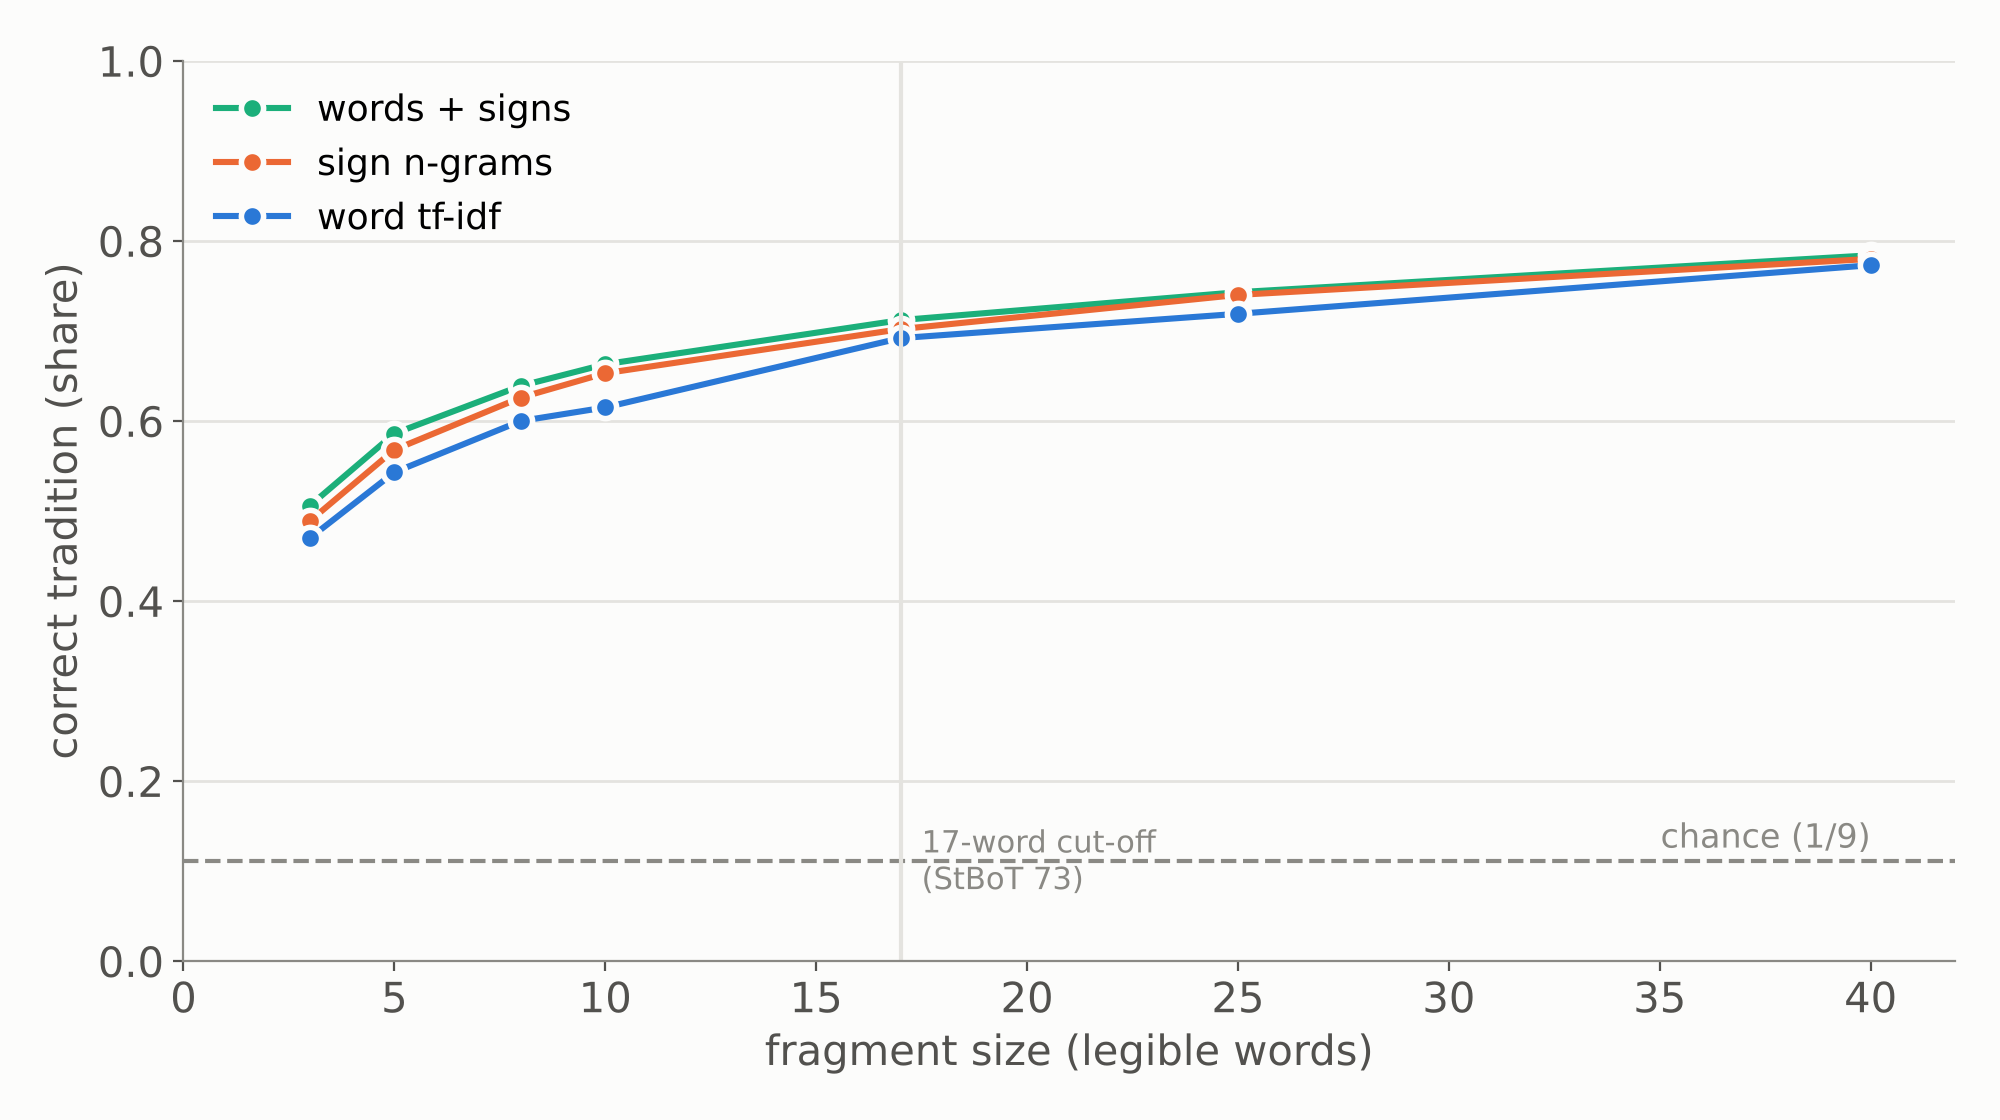
\includegraphics[width=0.8\linewidth]{coverage_curve.png}
  \caption{Accuracy of tradition assignment for held-out windows of $k$ legible words. The
    vertical line marks the 17-word cut-off of \cite{gordin2025matters}.}
  \label{fig:coverage}
\end{figure}

\subsection{What identifies a tradition: what is written, or how?}
\label{sec:layers}

Table~\ref{tab:layers} evaluates each layer alone. Content carries the identity of a tradition:
logograms reach \Q{E7.logograms.acc}, Hittite vocabulary \Q{E7.lexicon.acc}, and foreign-language
words \Q{E7.foreign.acc} in the \Q{E7.foreign.n} manuscripts that have them. The variable words
reach \Q{E7.spelling.acc} with their spelling kept and \Q{E7.collapsed.acc} with it collapsed:
the spelling choice adds nothing beyond the words themselves. The seven orthographic rates are a
weak but real signal, \Q{E7.orthographic_indices.acc} against \Q{E7.orthographic_indices.null_mean}
for shuffled labels ($p = \Q{E7.orthographic_indices.p}$).

\begin{table}[t]
  \caption{Each layer of a text alone: leave-one-manuscript-out accuracy over the reference
    traditions. $n$: manuscripts with at least one feature of the layer.}
  \label{tab:layers}
  \small
  \begin{tabular}{l r r r r}
    \toprule
    Layer & $n$ & majority & shuffled & accuracy \\
    \midrule
    \gentab{layers}
    \bottomrule
  \end{tabular}
\end{table}

The word classes of \cite{gordin2025matters} point the same way (Table~\ref{tab:wordclass}).
Removing function words, verbs or agents costs almost nothing (\Q{E8.all.words} with all words,
\Q{E8.without_function.words} without function words, \Q{E8.without_verb.words} without verbs):
these classes form a layer shared across traditions. Alone they still reach
\Q{E8.only_function.words} and \Q{E8.only_verb.words}, well above the majority baseline, so the
formulae differ between traditions, but less than realia (\Q{E8.only_realia.words}) or foreign
words (\Q{E8.only_foreign.words}). The previous study suggested that shared Akkadograms among
function words and verbs might reveal a writing habit \cite{gordin2025matters}; at the scale of
traditions, that layer is common ground rather than a marker.

\begin{table}[t]
  \caption{Word classes: accuracy with only that class, and with everything except it, in the
    word and sign spaces. Majority baseline for the class alone.}
  \label{tab:wordclass}
  \small
  \begin{tabular}{l r r r r r r}
    \toprule
    & & & \multicolumn{2}{c}{class alone} & \multicolumn{2}{c}{without class} \\
    \cmidrule(lr){4-5}\cmidrule(lr){6-7}
    Class & $n$ & majority & words & signs & words & signs \\
    \midrule
    \gentab{wordclass}
    \bottomrule
  \end{tabular}
\end{table}

\paragraph{Cultural and scribal profiles.}
The distinctive features of each tradition (Appendix~\ref{app:distinctive}) are ritual
materials, offerings, performers and deities: AZU, EREN and SÍSKUR in the Syro-Mesopotamian
group, SÍG and ZA.GÌN in the Kizzuwatna rituals, LUGAL and DUMU.É.GAL in the Hattian cult
layer. Spelling habits behave differently. The plene spelling \textit{me-ma-a-i} appears in
\Q{plene.memai.kizzuwatnalowerlandhurrian} Kizzuwatna--Lower Land manuscripts, all of them
\CTH{\Q{plene.memai.kizzuwatnalowerlandhurrian.cths}}, and \textit{pé-e-ra-an} in
\Q{plene.peran.luwianfestivalsistanuwalallupiya} Ištanuwa and Lallupiya manuscripts, all \CTH{\Q{plene.peran.luwianfestivalsistanuwalallupiya.cths}}.
Spelling habits attach to compositions and their copies, not to whole traditions. Inside
\CTH{701}, the orthographic rates do not predict script date either (\Q{E7date.acc} against a
majority of \Q{E7date.majority}), so there they are not merely a proxy for date. The
per-tradition rates are in Appendix~\ref{app:profile}.

\subsection{What is a fragment judged on?}
\label{sec:decision}
Looking at individual placements raises an obvious worry: the most common words of the corpus,
the particle \textit{nu} above all, weigh heavily in a fragment's similarity to its tradition. Since
the score is a cosine, the decision between the nearest tradition and the runner-up splits
exactly over the features, $\cos(x,c_1)-\cos(x,c_2)=\sum_f x_f\,(c_{1,f}-c_{2,f})$, and every
feature occurs in words whose class is known (the categories of \cite{gordin2025matters}). So each
decision can be divided into word categories and into layers: the word form, its syllabic signs,
and its logograms. Figure~\ref{fig:decision} compares the two quantities for the
\Q{E11a.texts} correctly placed reference manuscripts.

Similarity and decision differ. Features attested in at least a quarter of the reference texts
(\textit{nu} and single signs such as \textit{a} and \textit{i}) make up \Q{E11b.common.similarity}
of the similarity but only \Q{E11b.common.ref} of the decision, because they are shared by every
centroid and largely cancel. The 25 most frequent words carry \Q{E11b.frequent.similarity} of the
similarity and \Q{E11b.frequent.ref} of the decision. Deleting the 100 most frequent words
(\Q{E11c.k100.removed} of all word tokens: \Q{E11b.frequentlist}, \dots) leaves leave-one-out
accuracy at \Q{E11c.k100.acc} (\Q{E11c.k0.acc} with them), and deleting 200 at \Q{E11c.k200.acc}.
For whole manuscripts, then, the particles look decisive but are not.

\begin{figure}[t]
  \centering
  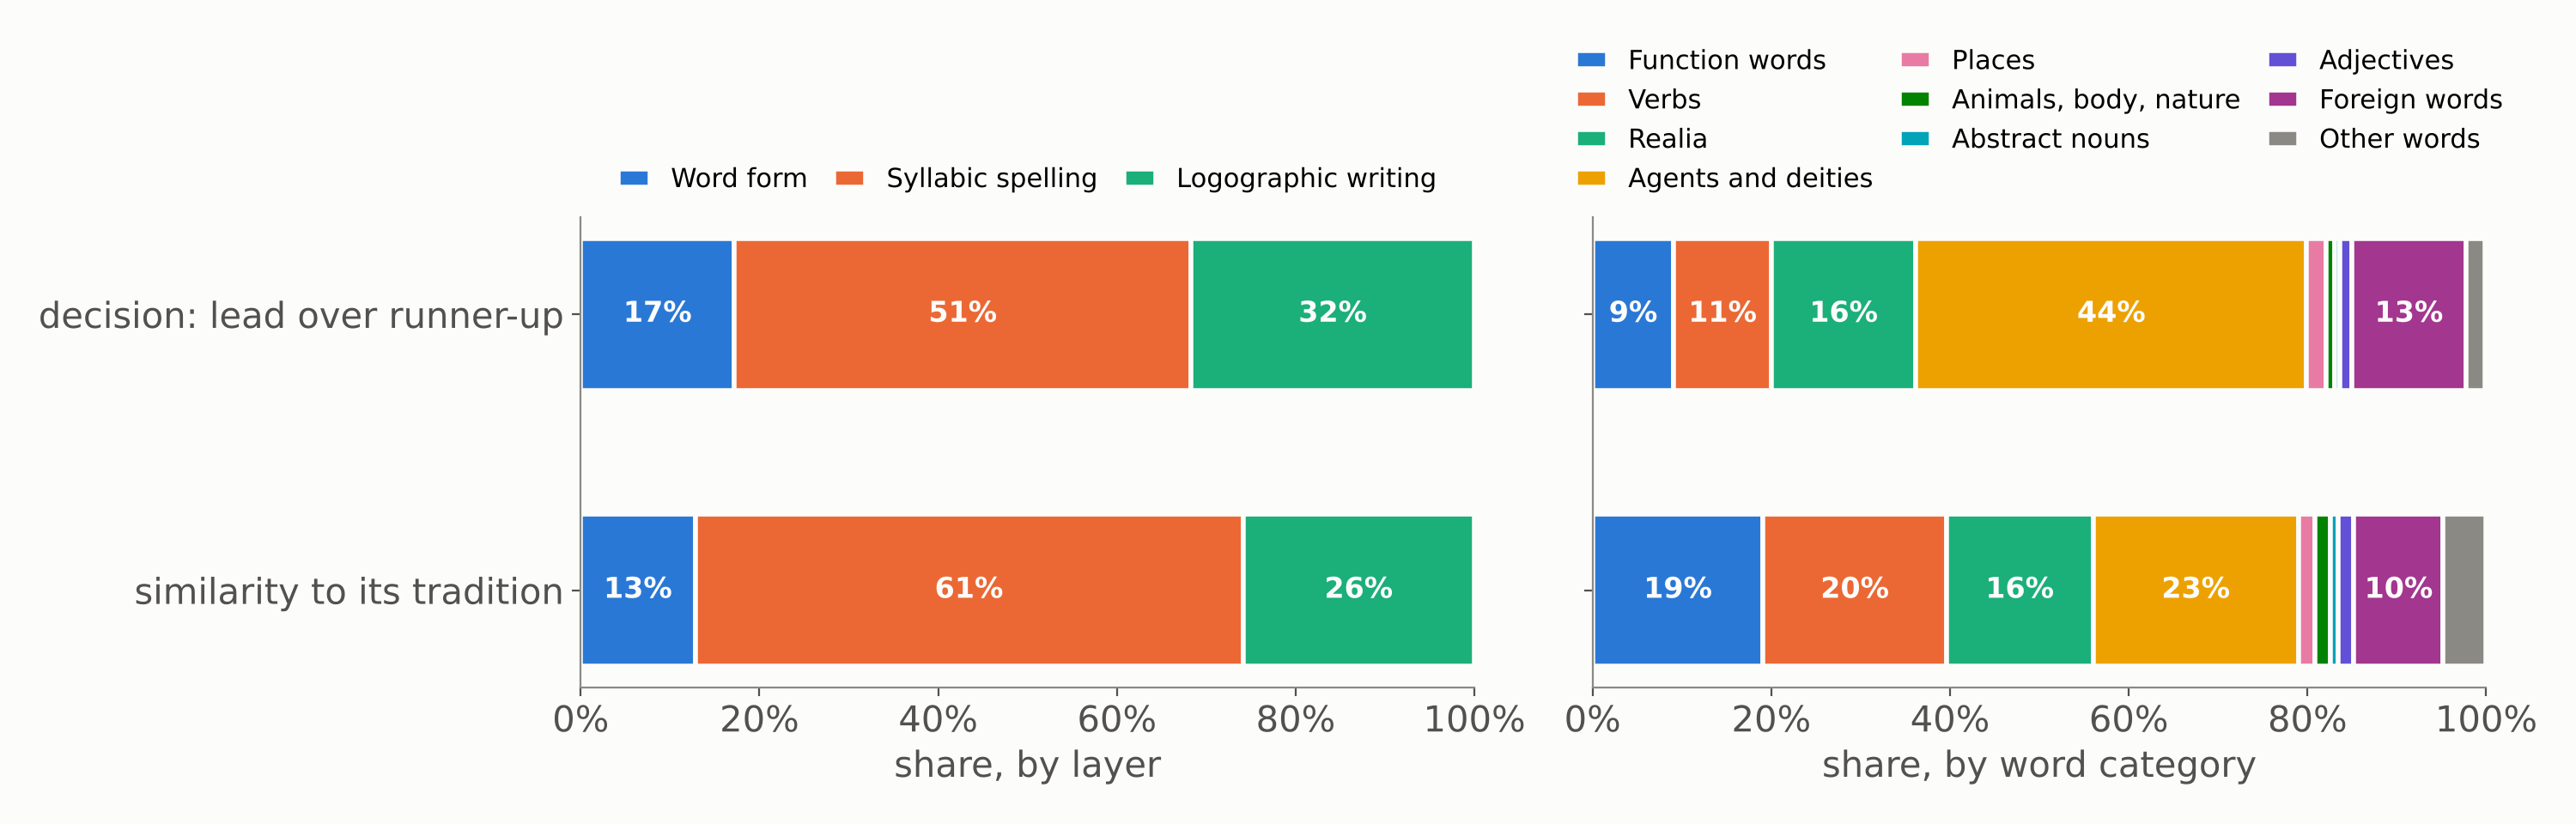
\includegraphics[width=\linewidth]{decision_shares.png}
  \caption{Similarity to the own tradition against the decision (lead over the runner-up), by
    layer and by word category, for the correctly placed reference manuscripts.}
  \label{fig:decision}
\end{figure}

The decision rests on content words: nouns and realia \Q{E11a.decision.nounsandrealia}, agents and
deities \Q{E11a.decision.agentsanddeities}, function words \Q{E11a.decision.functionwords}, verbs
\Q{E11a.decision.verbs} and foreign words \Q{E11a.decision.foreignwords}. Each tradition has its
own decisive category (Table~\ref{tab:decision}). The Ḫuwaššanna and Palaic festivals rest on
agents and deities (\Q{E11a.huwassannafestivals.agentsanddeities},
\Q{E11a.palaicfestivals.agentsanddeities}), Palaic also on Palaic words
(\Q{E11a.palaicfestivals.foreignwords}). The Kizzuwatna rituals rest on realia
(\Q{E11a.kizzuwatnarituals.nounsandrealia}: \Q{E11b.kizzuwatnarituals.features}). The Ištanuwa and
Lallupiya festivals rest on nouns, chiefly their own place names
(\Q{E11a.luwianfestivalsistanuwalallupiya.nounsandrealia}). Function words decide only where a
formula is particular to a group: in the Mixed group (\Q{E11a.mixedhurriansyrianluwian.functionwords}) the repetition mark KI.MIN and \textit{EGIR-anda-ma}
belong to how its festival lists are laid out. The common features, the negative column of the
table, often argue against the small traditions; the Hattian cult layer is the exception, where
they carry \Q{E11b.hattiancultlayer.common} of the decision and the leading features include
single syllabic signs (\Q{E11b.hattiancultlayer.features}). We take this to be its sign
distribution (plene vowels in particular, Appendix~\ref{app:profile}), and so the one tradition
where a scribal feature in the narrow sense helps decide; this reading is our inference from the
features, not a separate test.

\begin{table}[t]
  \caption{What the decision rests on, per tradition: share of the lead over the runner-up by
    word category and by layer, and the share carried by common features (in $\geq$25\% of
    reference texts), over the correctly placed manuscripts ($n$). Shares can be negative when a
    category argues for the runner-up; ``other words'' (not shown) completes the categories to
    100\%. Traditions with fewer than ten manuscripts are unstable.}
  \label{tab:decision}
  \footnotesize
  \setlength{\tabcolsep}{3pt}
  \begin{tabular}{l r r r r r r r r r r}
    \toprule
    & & \multicolumn{5}{c}{word category} & \multicolumn{3}{c}{layer} & \\
    \cmidrule(lr){3-7}\cmidrule(lr){8-10}
    Tradition & $n$ & funct. & verbs & nouns & agents & foreign & form & syll. & logo. & common \\
    \midrule
    \gentab{decision}
    \bottomrule
  \end{tabular}
\end{table}

\paragraph{Word categories and scribal features.}
By layer, syllabic signs carry \Q{E11a.decision.syllabicspelling} of the decision, logograms
\Q{E11a.decision.logographicwriting} and word forms \Q{E11a.decision.wordform}. This does not make
spelling the main signal: a syllabic sign n-gram carries the word it writes as well as the way it
is written. The spelling choice alone is isolated in Section~\ref{sec:layers}, where keeping or
collapsing the variant spellings changes accuracy from \Q{E7.collapsed.acc} to
\Q{E7.spelling.acc}. Word categories identify traditions; spelling and logographic habits, apart
from the Hattian case, attach to compositions and copies. The distinction the previous study drew
between what is written and how it is written \cite{gordin2025matters} holds at the level of the
decision as well.

\paragraph{When common words do decide.}
For short fragments the worry is justified. The share of the decision carried by common features
falls with length, from \Q{E11b.len510.common} for orphans of 5--10 words to
\Q{E11b.len50.common} above 50 words, and \Q{E11b.assigned_orphans_mostly_common} of the
\Q{E11b.assigned_orphans} placed orphans rest mostly on them. In windows cut from reference
manuscripts, such placements are right \Q{E11d.w5.common.prec}, \Q{E11d.w10.common.prec} and
\Q{E11d.w20.common.prec} of the time for 5, 10 and 20 words, against \Q{E11d.w5.rest.prec},
\Q{E11d.w10.rest.prec} and \Q{E11d.w20.rest.prec} for the rest. We therefore report the
decomposition with every placement, and treat one that rests mostly on common features as weak
whatever its margin.

\subsection{CTH 701 as a test bed}
\label{sec:cth701}

Salvini and Wegner's subgroups of the AZU rituals provide partial ground truth. On
\Q{E3.both.n} manuscripts in \Q{E3.both.classes} subgroups, the method recovers
\Q{E3.both.acc} of labels (words \Q{E3.words.acc}, signs \Q{E3.signs.acc}) against a majority
baseline of \Q{E3.both.majority} ($p = \Q{E3.both.p}$; Figure~\ref{fig:cth701}). The same
procedure does not predict script date: \Q{E3date.both.acc} against a majority of
\Q{E3date.both.majority} ($p = \Q{E3date.both.p}$). The subgroups are therefore not
script-date clusters. Removing the Hurrian and other foreign words lowers subgroup accuracy from
\Q{E8.701.all.words} to \Q{E8.701.without_foreign.words}, the largest drop of any class, yet
the remainder is still more than twice the majority baseline: the recitations carry the
subgroups, but the Hittite frame text differs between them as well. The \Q{E3.unclassified}
unclassified and group-f fragments are placed among groups a--e as candidate attributions in
the released tables.

\begin{figure}[t]
  \centering
  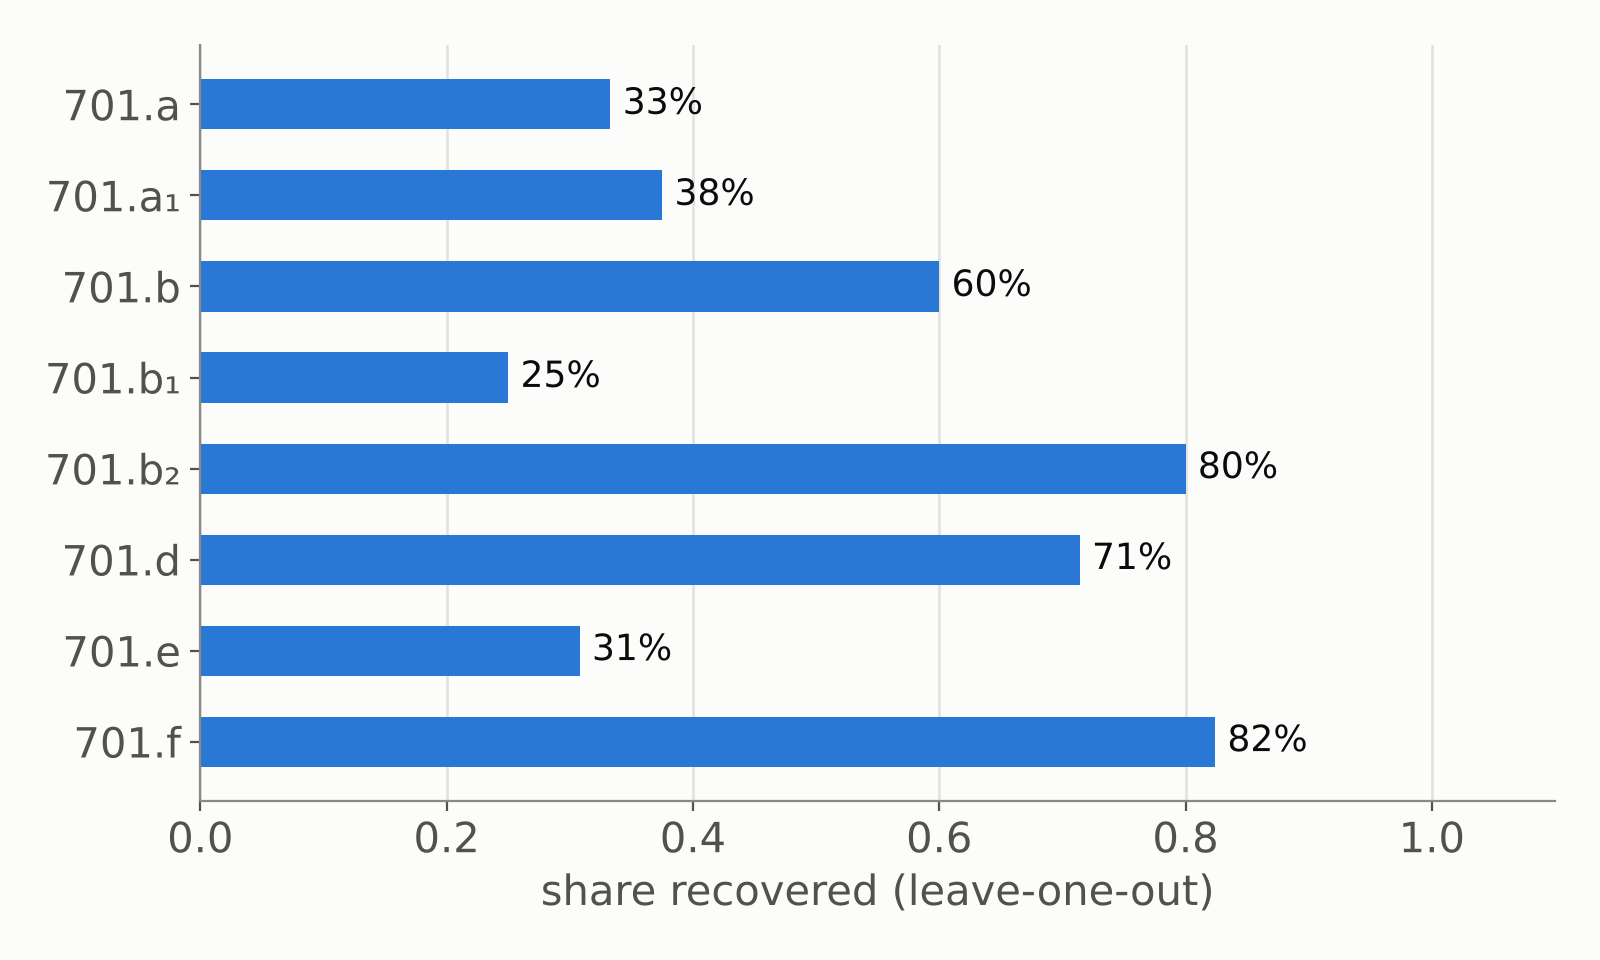
\includegraphics[width=0.75\linewidth]{cth701_subgroups.png}
  \caption{Recall of Salvini and Wegner's \CTH{701} subgroups, leave one manuscript out.}
  \label{fig:cth701}
\end{figure}

\subsection{Orphans placed}
\label{sec:orphans}

With the calibrated margin, \Q{E5.assigned} of the \Q{corpus.orphans_used} orphans are assigned
and \Q{E5.abstained} are left unassigned (\Q{E5.assigned.lo}--\Q{E5.assigned.hi} assigned
across the margin's 90\% interval; Figure~\ref{fig:orphans}). The \Q{E5.top} receive
\Q{E5.top.n} of them (\Q{E5.top.share}).

The two test sets show why that number needs care. The \CTH{390}--469 residue is placed mostly
with the Kizzuwatna rituals (\Q{E5b.res.kizz} of \Q{E5b.res.assigned} assigned), although no
study assigns these texts there: the Kizzuwatna rituals are the only large ritual class, so the
placement follows genre before origin. \CTH{500} behaves differently. Only \Q{E5b.c500.kizz} of
its \Q{E5b.c500.assigned} assigned fragments go to the Kizzuwatna rituals and
\Q{E5b.c500.hurrian} to the Hurrian festival groups, which agrees with HFR's treatment of
\CTH{500} as festival material \cite{hfr}.

\begin{figure}[t]
  \centering
  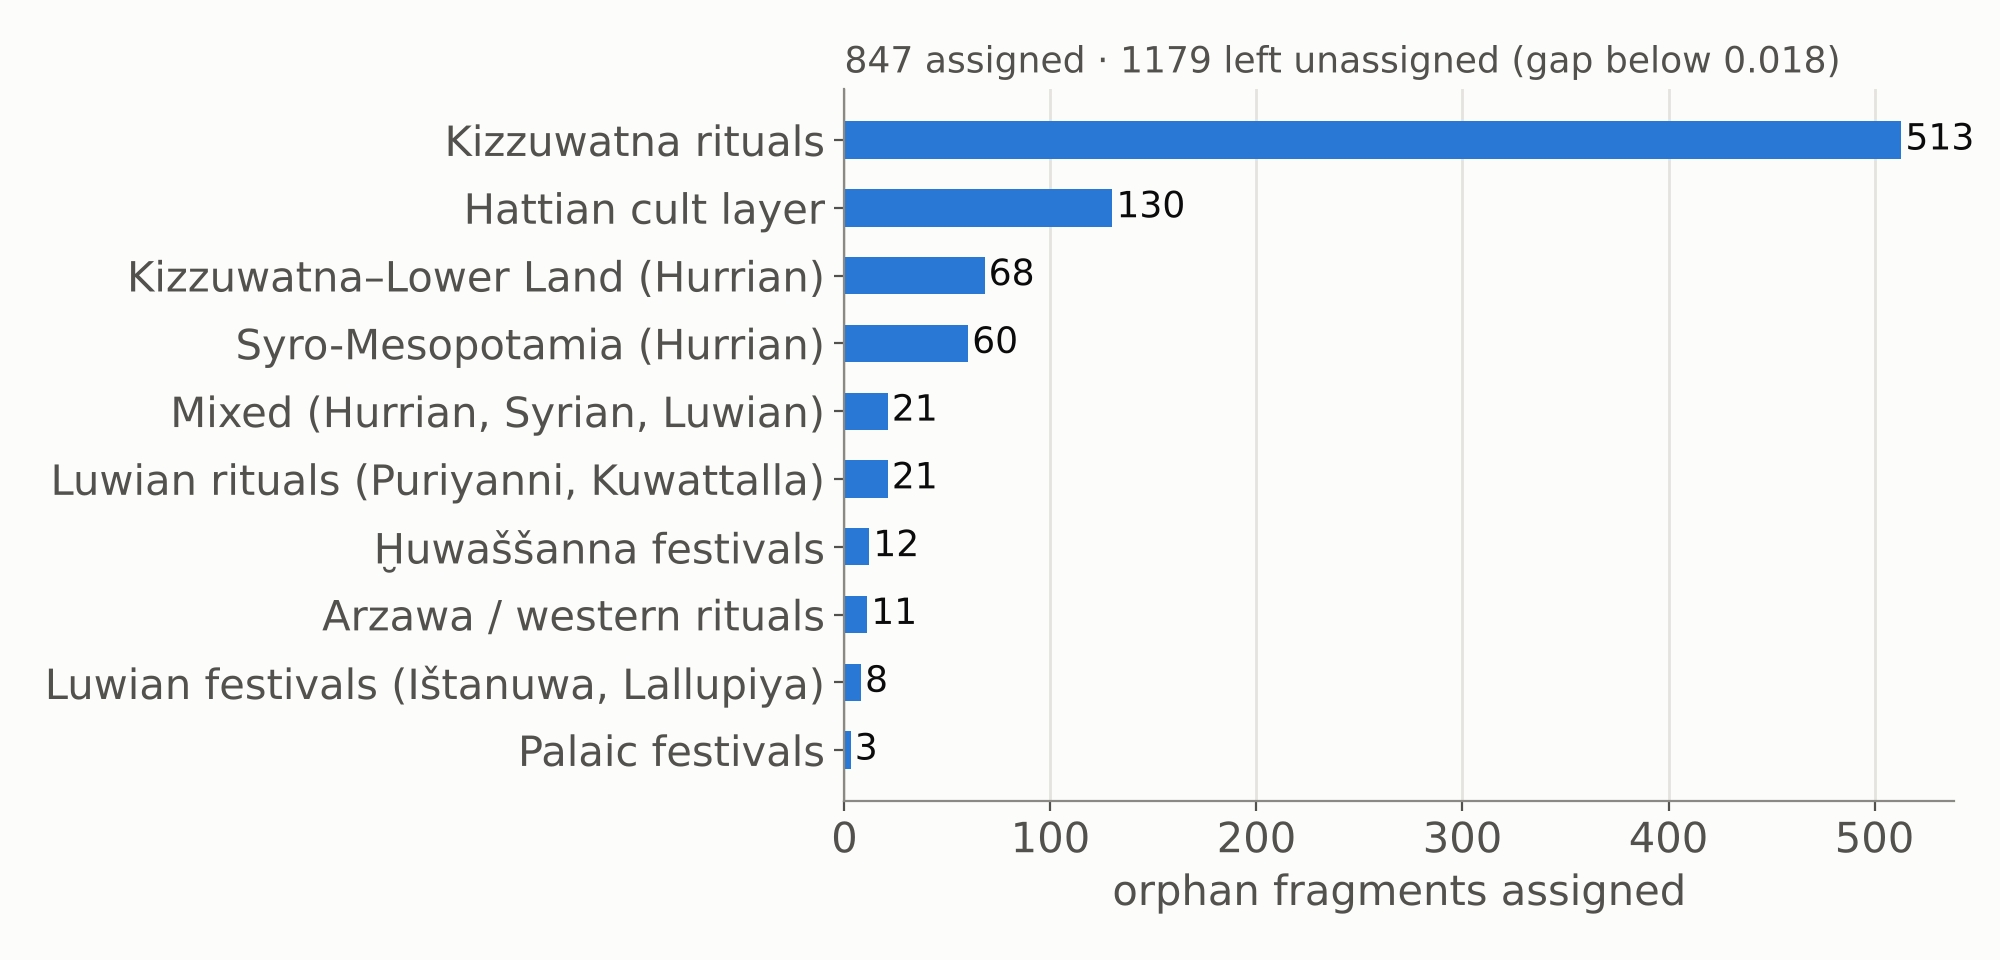
\includegraphics[width=0.8\linewidth]{orphans_by_tradition.png}
  \caption{Orphans (\CTH{470} and EBo, five or more legible words) assigned to each tradition
    above the calibrated margin.}
  \label{fig:orphans}
\end{figure}

\subsection{Does a fragment fit any known tradition?}
\label{sec:openset}

Table~\ref{tab:openset} shows that the margin rule is fooled by texts from outside the
reference. At \Q{E9.k} words, it still places \Q{E9.genres.placed.lo}--\Q{E9.genres.placed.hi}
of the windows from the \Q{E9.genres.count} other genres in some tradition, and
\Q{E9.fest.placed} of the windows from festivals of other traditions. A floor on similarity
separates other genres fairly well (AUROC \Q{E9.genres.auroc.lo}--\Q{E9.genres.auroc.hi}) but
not other festivals (\Q{E9.fest.auroc}). A genre gate works better: with the outside genres as
classes of their own, \Q{E9.genres.gate.lo}--\Q{E9.genres.gate.hi} of their windows and
\Q{E9.fest.gate} of the other festivals are recognised as outside, at the cost of sending
\Q{E9.ref.gate} of reference windows away. The Luwian rituals of Taurisa are placed in \Q{E9.luwianritualsoftaurisa.placed} of
windows and recognised by the gate in \Q{E9.luwianritualsoftaurisa.gate_sent_outside}, but rest
on only \Q{E9.luwianritualsoftaurisa.texts} texts.

\begin{table}[t]
  \caption{Open-set test, windows of \Q{E9.k} words, five folds. Placed: share passing the
    margin rule (wrongly, for outside texts). AUROC: separation of reference and outside
    windows by top similarity. Gate: share whose nearest class is an outside genre.}
  \label{tab:openset}
  \small
  \begin{tabular}{l r r r r}
    \toprule
    Texts & $n$ & placed & AUROC & gate \\
    \midrule
    \gentab{openset}
    \bottomrule
  \end{tabular}
\end{table}

Applied to the orphans, the gate finds \Q{E9.orph.outside} of \Q{E9.orph.scored} that are closer
to an outside genre than to any tradition by more than the margin; \Q{E9.orph.assigned_outside}
of them had been assigned. Most are Hattian-layer placements that look like festivals of other
traditions (\Q{E9.orph.hattiancultlayer.festivalsofothertraditions}) and Kizzuwatna placements that
look like myths (\Q{E9.orph.kizzuwatnarituals.myths}) or instructions
(\Q{E9.orph.kizzuwatnarituals.instructions}). They are released as candidates for re-filing.

%% ==========================================================================================
\section{Quantitative Scribal Tradition Mapping}
\label{sec:qtm}

The results suggest a division of labour between two levels of a text, which QTM makes
explicit. Borrowing the terms of textual criticism \cite{maas1958textual,trovato2014lachmann},
a tradition is treated as an \term{archetype}: not a reconstructed text, but the body of
vocabulary, formulae and foreign-language recitation that its manuscripts share. Each
manuscript, and each orphan, is a \term{witness} that attests a part of it. What identifies the
archetype is its content: the layers that carry tradition in Section~\ref{sec:layers} are the
cultural ones. What marks the witness is its spelling: plene habits and orthographic rates
cluster by composition and copying line, not by tradition, which agrees with the view that
Hittite writing habits belong to scribal circles and their schooling \cite{gordin2015scribal}.
Logograms sit on both sides: the object named is cultural, the decision to write it
logographically is scribal \cite{weeden2011logograms}.

An orphan is a low-coverage witness. Coverage, the share of a tradition's 200 core terms that
its assigned orphans attest, is near complete for the traditions that receive many orphans
(\Q{trad.kizzuwatnarituals.coverage} for the Kizzuwatna rituals, \Q{trad.hattiancultlayer.coverage}
for the Hattian layer) and low for those that receive few (\Q{trad.palaicfestivals.coverage} for
the Palaic festivals with \Q{trad.palaicfestivals.orphans} orphans). In its present form this
measure grows with the number of orphans, so it cannot yet be compared across traditions;
rarefaction to equal orphan counts \cite{gotelli2001rarefaction}, and unseen-species estimates of
the kind applied to lost medieval literature \cite{kestemont2022forgotten}, are the natural next
steps. Read this way, the question becomes historical: which traditions circulated widely in
copies that now survive only as fragments, and which are known almost only from their
identified compositions.

%% ==========================================================================================
\section{Discussion and limitations}
\label{sec:discussion}

\paragraph{Genre before origin.}
The residue result shows the main risk of the method. A fragment is placed by what it shares
with the reference, and the largest shared layer is genre. A Hittite ritual from outside every
reference tradition will look most like the largest ritual class. The open-set test shows the
same risk across genres. A placement should therefore be read as ``nearest of these'' unless the
reference includes the plausible alternatives as classes. The genre gate is a first step, and
each new tradition narrows the gap: with the Luwian rituals of \CTH{758}--763 in the reference,
\Q{E5b.res.luwianritualspuriyannikuwattalla} residue texts are placed with them rather than with
a larger ritual class.

\paragraph{Limitations.}
TLHdig's normalised forms are uneven across editors, and broken words are dropped, so short
fragments over-represent formulaic lines, and their placements rest more on common features
(Section~\ref{sec:decision}). The idf weights are fitted on the whole reference
set. Several traditions are small (\Q{trad.smallest} has \Q{trad.smallest.n} test manuscripts),
and their recall is uncertain; held out by composition, several of them are not recovered at all (Section~\ref{sec:recovery}). Festival manuscripts differ by function (outline tablets, day
tablets, cult inventories close to festival text \cite{cammarosano2021inventories}), which word
profiles may track alongside tradition. The Hattian layer's preference for plene writing and few
logograms may reflect Old Hittite manuscripts as much as tradition, and is still to be checked
against script dates. Finally, every placement is a hypothesis for philological verification on
the tablet: an orphan placed near a known manuscript is a candidate join, not a join.

%% ==========================================================================================
\section{Conclusion}
\label{sec:conclusion}

Content-based assignment places Hittite ritual fragments in literature-defined traditions well
above chance, from about ten legible words on, and recovers subgroup structure inside \CTH{701}
without being a proxy for script date. The signal lies in what is written; spelling marks the
copying line. A closed reference over-assigns, and the open-set test shows how to make the
abstention honest. QTM turns these observations into a programme: orphans as witnesses, traditions
as archetypes, and coverage as the measure of how much of a tradition survives only in
fragments.

%% ==========================================================================================
\section{Data and code availability}
\label{sec:availability}

Code, the frozen \CTH{701} label snapshot and all outputs are in the repository
\url{https://github.com/shaigordin/measuring-scribal-literacy} (folder \texttt{orphans/}).
\texttt{reproduce.sh} downloads TLHdig 0.3 from Zenodo, verifies its checksum and rebuilds every
experiment, figure and table; all randomness is seeded and a rerun is byte-identical. The paper
itself (\texttt{paper/}) is generated from those outputs: \texttt{make\_numbers.py} writes every
number in the text and every results table, and \texttt{generated/numbers\_index.csv} lists each
number with the file and field it comes from.

\begin{acknowledgments}
  We thank the TLHdig and HFR teams of the Akademie der Wissenschaften und der Literatur Mainz
  and the Universities of Würzburg and Marburg, whose openly licensed corpus made this study
  possible. % TODO: funding and colleagues
\end{acknowledgments}

\section*{Declaration on Generative AI}
During the preparation of this work, the author used Claude (Anthropic) in order to: write and
run the analysis code, draft the text, and check bibliographic references. After using this
tool, the author reviewed and edited the code and the content as needed and takes full
responsibility for the publication's content.
% TODO (author): confirm or adjust this declaration (CEUR-WS GenAI policy, ceur-ws.org/genai-tax.html)

\bibliography{references}

\appendix

\section{Distinctive features per tradition}
\label{app:distinctive}

\begin{table*}[h]
  \caption{The four most distinctive features of each tradition per layer (weighted log-odds
    with an informative prior \cite{monroe2008fightin}, on manuscript frequencies), as TLHdig
    forms. Full lists in \texttt{E7\_distinctive\_features.csv}.}
  \small
  \begin{tabularx}{\textwidth}{>{\raggedright}p{0.2\textwidth} >{\raggedright}X >{\raggedright}X
      >{\raggedright\arraybackslash}X}
    \toprule
    Tradition & Logograms & Hittite vocabulary & Foreign words \\
    \midrule
    \gentab{distinctive}
    \bottomrule
  \end{tabularx}
\end{table*}

\section{Orthographic profiles}
\label{app:profile}

\begin{table*}[h]
  \caption{Mean orthographic rates per tradition as $z$-scores over all reference manuscripts:
    shares of logograms, Akkadograms, phonetic complements, determinatives, plene spellings,
    CVC signs and \textit{ú}.}
  \small
  \begin{tabular}{l r r r r r r r}
    \toprule
    \gentab{profile}
    \bottomrule
  \end{tabular}
\end{table*}

\end{document}
